\documentclass{article}

\usepackage[utf8]{inputenc}
\usepackage[russian]{babel}
\usepackage{graphicx}
\graphicspath{{results/}}
\DeclareGraphicsExtensions{.pdf,.png,.jpg}
\usepackage[unicode, pdftex]{hyperref}
\usepackage{csvsimple}
\usepackage[stable]{footmisc}
\usepackage{subfigure}
\usepackage{indentfirst}


\begin{document}

\begin{titlepage}
  \centerline {Санкт-Петербургский политехнический университет}
  \centerline { им. Петра Великого}
  \centerline { }
  \centerline {Институт прикладной математики и механики} 
  \centerline {Кафедра "Прикладная математика"}
  \vfill
  \centerline{\textbf{Отчёт}}
  \centerline{\textbf{по лабораторной работе №6}}
  \centerline{\textbf{по дисциплине}}
  \centerline{\textbf{"Математическая статистика"}}
  \vfill
  \hfill
  \begin{minipage}{0.45\textwidth}
  Выполнил студент:\\
  Дроздова Дарья Александровна\\
  группа: 3630102/80401 \\
  \\
  Проверил:\\
  к.ф.-м.н., доцент \\
  Баженов Александр Николаевич
  \end{minipage}
  \vfill
  \centerline {Санкт-Петербург}   
  \centerline {2021 г.}  
\end{titlepage}

\newpage
\setcounter{page}{2}
\tableofcontents

\newpage
\listoffigures

\newpage
\section{Постановка задачи}

Найти оценки коэффициентов линейной регрессии
$$
y_i = a + bx_i + e_i
$$
используя 20 точек на отрезке $[-1.8; 2]$ с равномерным шагом равным 0.2. Ошибку $e_i$ считать нормально распределенной с параметрами $(0, 1)$. \\ 

В качестве эталонной зависимости взять
$$
y_i = 2 + 2x_i + e_i
$$ 

При построении оценок коэффициентов использовать два критерия: критерий наименьших квадратов и критерий наименьших модулей. \\

Проделать аналогичную процедуру для выборки с возмущением:
$$
y_1 = y_1 + 10, \; y_{20} = y_{20} - 10
$$

\newpage
\section{Теория}

\subsection{Модель простой линейной регрессии}

Регрессионную модель описания данных называют линейной регрессией, если
$$
y_i = \beta_0 + \beta_1x_i+\varepsilon_i, \;\; i=1,...,n
$$
где $x_1,...,x_n$ - заданные числа, $y_1,...,y_n$ - наблюдаемые значения отклика, $\varepsilon_1,...,\varepsilon_n$ - независимые, нормально распределенные $N(0, \sigma)$ с нулевым математическим ожиданием и одинаковой дисперсией случайные величины, $\beta_0, \beta_1$ - неизвестные параметры, подлежащие сравнению.

\subsection{Метод наименьших квадратов}

Метод наименьших квадратов один из самых распространенных методов оценки параметров регрессионной модели. Метод заключается в следующем: вводится критерий рассогласованности отклика и регрессионной функции, и оценки параметров регрессии определяются так, чтобы сделать это рассогласование наименьшим. Достаточно простые расчетные формулы для оценок получают при выборе критерия в виде суммы квадратов отклонений значений отклика от значений регрессионной функции:
\begin{equation}
Q(\beta_0, \beta_1) = \sum^n_{i=1} \varepsilon^2_i = \sum^n_{i=1}(y_i - \beta_0 - \beta_1x_i)^2 \to \min_{\beta_0, \beta_1}
\label{eq:1}
\end{equation}

\subsubsection{Расчетные формулы для МНК-оценок}

МНК-оценки параметров $\widehat{\beta_0},\widehat{\beta_1}$ находятся из условия обращения функции (\ref{eq:1}) в минимум. \\

Из необходимых условий экстремума можно вывести следующие оценки:
\begin{equation}
\widehat{\beta_1} = \frac{\overline{xy} - \overline{x}\overline{y}}{\overline{x^2} - (\overline{x})^2}
\label{eq:2}
\end{equation}
\begin{equation}
\widehat{\beta_0} = \overline{y} - \overline{y}\widehat{\beta_1}
\label{eq:3}
\end{equation}

\subsection{Метод наименьших модулей}

В качестве альтернативы для метода наименьших квадратов используют метод наименьших модулей, который заключается в поиске минимума следующей функции
$$
\sum^n_{i=1} | y_i - \beta_0 - \beta_1x_i | \to \min_{\beta_0, \beta_1}
$$

\subsubsection{Расчетные формулы для МНМ-оценок}

Из преобразования оценок $\widehat{\beta_1}, \widehat{\beta_0}$ можно вывести следующие МНМ-оценки
\begin{equation}
\widehat{\beta}_{1R} = r_q \frac{q^*_y}{q_x^*}
\label{eq:4}
\end{equation}
\begin{equation}
\widehat{\beta}_{0R} = \mathrm{med} \; y - \widehat{\beta}_{1R} \mathrm{med} \; x
\label{eq:5}
\end{equation}
где $r_Q$ - знаковый коэффициент корреляции, который определяется по формуле
$$
r_Q = \frac{1}{n} \sum^n_{i=1} \mathrm{sgn}(x_i - \mathrm{med} \; x) \; \mathrm{sgn}(y_i - \mathrm{med} \; y)
$$
$q_x^*, q_y^*$ - интерквартильные широты
$$
q_x^* = \frac{y_{(j)} - y_{(l)}}{k_q(n)}, \; q_x^* = \frac{x_{(j)} - x_{(l)}}{k_q(n)}
$$
$$
\left \{ \begin{array} {rcl}
[n/4] + 1 \qquad \mbox{при $n/4$ дробном} \\
n/4 \qquad \mbox{при $n/4$ целом} \\
\end{array} \right .
$$
$$
j = n - l + 1
$$


\newpage
\section{Реализация}

Лабораторная работа выполнена на языке программирования Python в среде разработки PyCharm. Для методов МНК и МНМ используется библиотека numpy и scipy для построений графиков - pyplot.

Код программы расположен в репозитории GitHub по ссылке: \url{https://github.com/Drozdova-Daria/Math_Stat_Lab6}

\newpage
\section{Результаты}

\subsection{Выборка без возмущений}

\begin{itemize}
	\item Критерий наименьших квадратов (\ref{eq:2}), (\ref{eq:3}):
	$$
	\widehat{a} = 1.87670, \; \widehat{b} = 2.13581
	$$
	\item Критерий наименьших модулей (\ref{eq:4}), (\ref{eq:5}):
	$$
	\widehat{a} = 1.92702, \; \widehat{b} = 2.22954
	$$
\end{itemize}

\begin{figure}[h]
\center{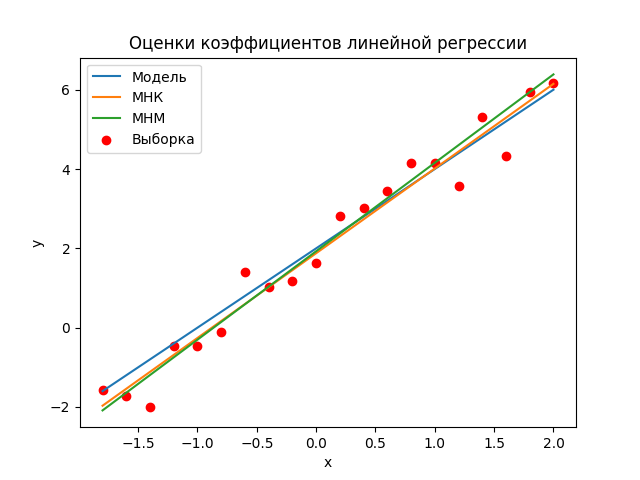
\includegraphics[scale=0.8]{1}}
\caption{Результат для выборки без возмущений}
\label{i:1}
\end{figure}

\newpage
\subsection{Выборка с возмущениями}

\begin{itemize}
	\item Критерий наименьших квадратов (\ref{eq:2}), (\ref{eq:3}):
	$$
	\widehat{a} = 2.01956, \; \widehat{b} = 0.70724
	$$
	\item Критерий наименьших модулей (\ref{eq:4}), (\ref{eq:5}):
	$$
	\widehat{a} = 1.92701, \; \widehat{b} = 2.22954
	$$
\end{itemize}

\begin{figure}[h]
\center{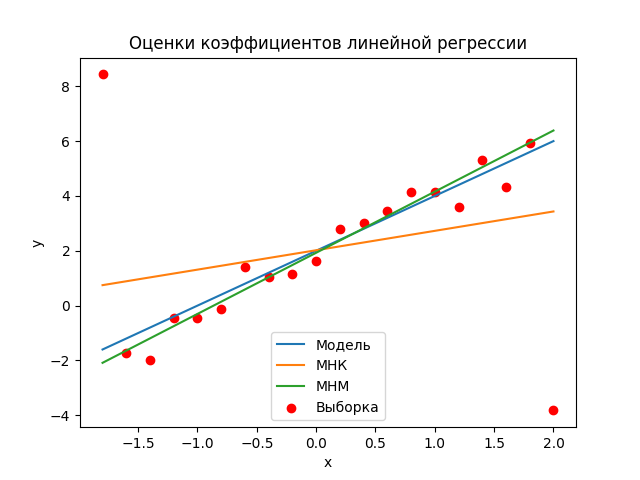
\includegraphics[scale=0.8]{2}}
\caption{Результат для выборки с возмущениями}
\label{i:2}
\end{figure}

\newpage
\section{Обсуждение}

Исходя из Рис. \ref{i:1} можно сказать, что критерий наименьших квадратов наиболее точно оценивает коэффициенты линейной регрессии на выборке без возмущений. По Рис. \ref{i:2} видно, что метод наименьших модулей точнее оценивает коэффициенты линейной регрессии на выборке с возмущениями.

\end{document}